\documentclass{beamer}

\usepackage[utf8]{inputenc}
\usecolortheme{beaver}
\usepackage{caption}
\usepackage{subcaption}
\usepackage{mathtools}
\usepackage{todonotes}
\usepackage{amsmath}
\usepackage{bm}
\usepackage{listings}
\usepackage{ragged2e}
\usepackage{titlecaps}
\usepackage{fancyvrb}

\def\ci{\perp\!\!\!\!\!\perp}

\newtheorem{proposition}{Proposition}
\Addlcwords{for a is but and with of in as the etc on to if}

\newcommand\github{
\includegraphics[height=3ex]{imgs/github.png}}
\newcommand\email{
\includegraphics[height=3ex]{imgs/email.png}}

\setbeamertemplate{section in toc}{\inserttocsectionnumber.~\inserttocsection}
\usetheme{Boadilla}
\makeatletter
\setbeamertemplate{footline}{%
    \leavevmode%
    \hbox{%
        \begin{beamercolorbox}[wd=.3\paperwidth,ht=2.25ex,dp=1ex,center]{author in head/foot}%
            \usebeamerfont{author in head/foot}\insertshortauthor\expandafter\beamer@ifempty\expandafter{\beamer@shortinstitute}{}{~~(\insertshortinstitute)}
        \end{beamercolorbox}%
        \begin{beamercolorbox}[wd=.55\paperwidth,ht=2.25ex,dp=1ex,center]{title in head/foot}%
            \usebeamerfont{title in head/foot}\insertshorttitle
        \end{beamercolorbox}%
        \begin{beamercolorbox}[wd=.15\paperwidth,ht=2.25ex,dp=1ex,right]{date in head/foot}%
            \usebeamerfont{date in head/foot}\insertshortdate{}\hspace*{2em}
            \insertframenumber{} / \inserttotalframenumber\hspace*{2ex} 
        \end{beamercolorbox}}%
        \vskip0pt%
    }
\makeatother

\begin{document}

\title[Causal Inference using pgmpy]{Introduction to Casual Inference using pgmpy}
\author{Ankur Ankan}
\institute[]{Postdoctoral Researcher \\ Radboud University, The Netherlands}
\date{}

\maketitle

\begin{frame}{Predictive vs Causal Modelling}
\end{frame}

\begin{frame}{Motivating Examples}
	\begin{itemize}
		\item Finding how variables interact.
		\item Key drivers of an outcome.
		\item Feature Selection
	\end{itemize}
\end{frame}

\begin{frame}{Motivating Examples}
\end{frame}

\begin{frame}{Motivating Examples}
\end{frame}

\begin{frame}{Two Main Framworks}
	Mathematical formulations of causal inference:
	\vspace{0.5em}
	\begin{itemize}
		\item Potential Outcomes Framework (a.k.a. Rubin's Casual Model)
			\begin{itemize}
				\item Counterfactual statement at the core.
				\item Provides statistical methods for estimating the counterfactual.
				\item Statistically robust methods that can deal with assumption violations.
			\end{itemize}
	\end{itemize}
	\vspace{2em}
	\begin{itemize}
		\item Directed Acyclic Graphs (DAGs) / Structural Equation Models (SEMs)
			\begin{itemize}
				\item Causal diagram, i.e., DAG at the core.
				\item Causal effect estimators can be defined using the DAG.
				\item Modelling assumptions are explicit.
			\end{itemize}
	\end{itemize}
\end{frame}

\begin{frame}{Landscape of Causal Inference Python Packages}
	\begin{columns}
		\begin{column}{0.5 \textwidth}
			\center{\textbf{Potential Outcomes Framework}}
			\begin{itemize}
				\item Estimation methods such as Propensity Score.
					\begin{figure}
						
\includegraphics[scale=0.2]{imgs/dowhy.png}
					\end{figure}
				\item Doubly Robust Estimation
					\begin{figure}
						
\includegraphics[scale=0.1]{imgs/doubleml.png}
					\end{figure}
				\item Meta Learners: T/S/X-Learners.
					\begin{figure}
						
\includegraphics[scale=0.3]{imgs/causalml.png}
					\end{figure}
			\end{itemize}

		\end{column}
		\vrule
		\begin{column}{0.5 \textwidth}
			\center{\textbf{DAG Framework}}
			\begin{itemize}
				\item pgmpy
					\begin{figure}
						
\includegraphics[scale=0.2]{imgs/pgmpy.png}
					\end{figure}
				\item \textbf{bnlearn}: Easy to use API
				\item casualnex
					\begin{figure}
						
\includegraphics[height=2cm, width=3cm, scale=0.2]{imgs/causalnex.png}
					\end{figure}
			\end{itemize}
		\end{column}
	\end{columns}
\end{frame}

\begin{frame}{A General Workflow in the DAG Framework}
	\begin{figure}
		\centering
		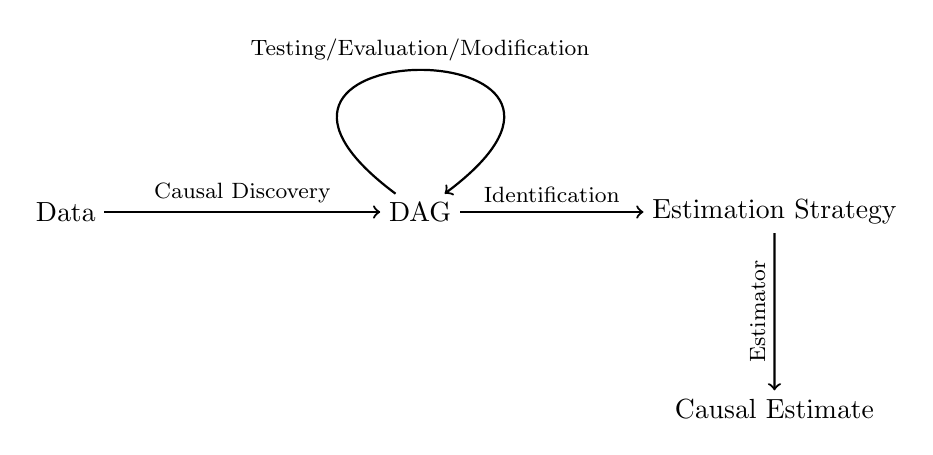
\begin{tikzpicture}[yscale=1, xscale=0.75, inner sep=3pt]
		\tikzstyle{every node}=[align=left]
			\node (data) at (0, 0) {Data};
			\node (dag) at (6, 0) {DAG};
			\node (estimand) at (12, 0) {Estimation Strategy};
			\node (estimation) at (12, -2.5) {Causal Estimate};
	
			\draw[thick, ->] (data) to node[midway, above]{\footnotesize Causal Discovery} (dag);
			\draw[thick, ->] (dag) to node[midway, above] {\footnotesize Identification} (estimand);
			\draw[thick, ->] (estimand) to node[midway, above, rotate=90] {\footnotesize Estimator} (estimation);
			\draw[thick, ->] (dag) [out=150, in=30, looseness=10] to node[midway, above] {\footnotesize Testing/Evaluation/Modification} (dag);
		\end{tikzpicture}
		\label{fig:workflow}
	\end{figure}
\end{frame}

\begin{frame}{What does pgmpy provide}
	\begin{itemize}
		\item Provides standardized implementations of commonly used algorithms.
		\item Practical methods methods.
		\item Extensible.
	\end{itemize}
\end{frame}

\begin{frame}{Causal Discovery}
	\begin{figure}
		\centering
		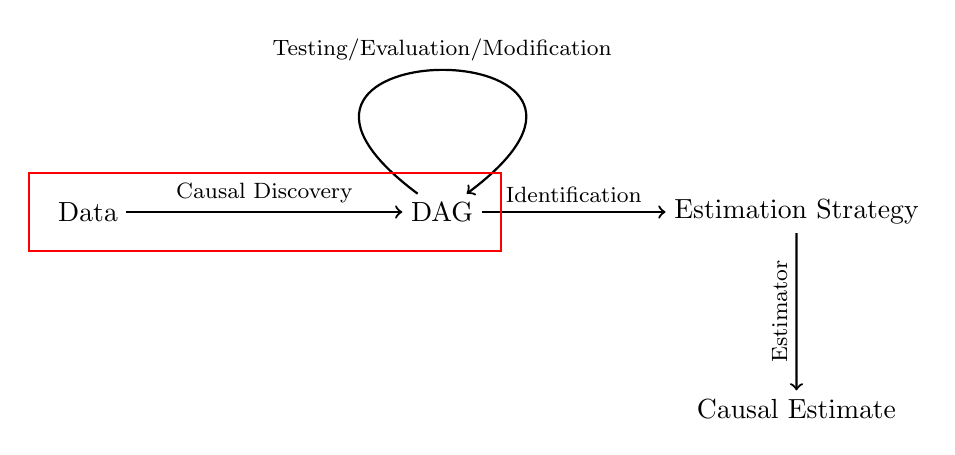
\begin{tikzpicture}[yscale=1, xscale=0.75, inner sep=3pt]
		\tikzstyle{every node}=[align=left]
			\node (data) at (0, 0) {Data};
			\node (dag) at (6, 0) {DAG};
			\node (estimand) at (12, 0) {Estimation Strategy};
			\node (estimation) at (12, -2.5) {Causal Estimate};
	
			\draw[thick, ->] (data) to node[midway, above]{\footnotesize Causal Discovery} (dag);
			\draw[thick, ->] (dag) to node[midway, above] {\footnotesize Identification} (estimand);
			\draw[thick, ->] (estimand) to node[midway, above, rotate=90] {\footnotesize Estimator} (estimation);
			\draw[thick, ->] (dag) [out=150, in=30, looseness=10] to node[midway, above] {\footnotesize Testing/Evaluation/Modification} (dag);

			\draw[draw=red, thick] (-1, -0.5) rectangle (7, 0.5);
		\end{tikzpicture}
		\label{fig:workflow1}
	\end{figure}
	\vspace{2em}
	\center \textbf{Casual Discovery: } Learn the causal structure among the variables using data.
\end{frame}

\begin{frame}{Automated Algorithms}
	\begin{itemize}
		\item Plenty of automated algorithms with nice asymptotic properties.
		\item In practice, output varies significantly depending on sample size,
			algorithm, and their hyperparameters.
		\item Difficult to decide which model is correct.
	\end{itemize}

\end{frame}

\begin{frame}{Automated Algorithms}
	\todo[inline]{Code for both}
	\center{\textbf{PC}: Constraint-Based Algorithm}
	\begin{figure}
		\centering
		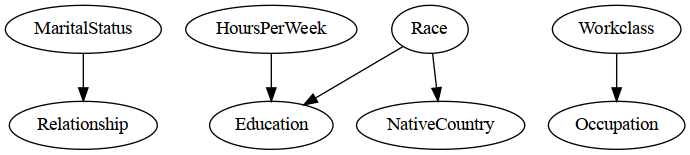
\includegraphics[scale=0.25]{imgs/adult_x2.png}
	\end{figure}
	\center{\textbf{Hill-Climb Search: } Score Based Algorithm}
	% \begin{figure}
	% 	\centering
	% 	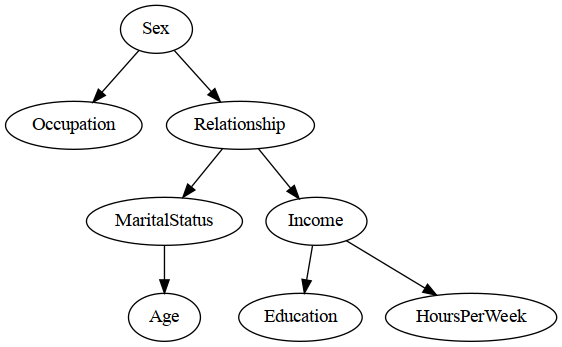
\includegraphics[scale=0.25]{imgs/adult_bic.png}
	% \end{figure}
\end{frame}

% \begin{frame}{PC algorithm}
% 	Constraint-Based Algorithm: Exploits Conditional Indpendences in the data to construct the DAG.	
% \end{frame}
% 
% \begin{frame}{Hill-Climb Search}
% 	Score based: Tries to optimize the score by doing local changes.
% 
% 	Results can be very different depending on the algorithm, hyperparameter selections, etc.
% \end{frame}

\begin{frame}{And it continues}
	\begin{figure}
		\centering
		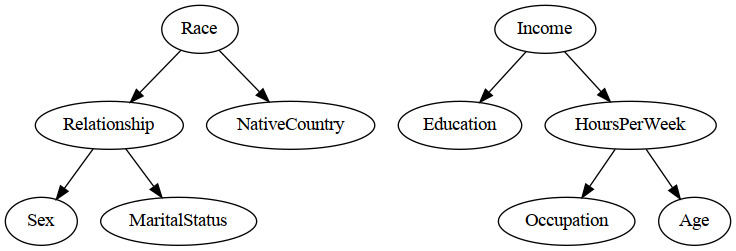
\includegraphics[scale=0.4]{imgs/adult_pillai.png}
	\end{figure}
\end{frame}

\begin{frame}{Casual Discovery}
	\center{Which of these models are correct?}

	\center{\textcolor{Probably None}}

	\center{Models learnt using algorithms are usually incorrect.}

	\center{\textcolor{red}{ How do we improve the output?}}

	\vspace{2em}

	\begin{itemize}
		\item Incorporate expert knowledge
		\item Testing models and manually modify based on that.
		% \item Really have to remember that: "All models are wrong, but some are useful" - George Box
		% \item Many automated algorithms but most of them would make mistakes.
		% \item Usually need to have some manual intervention. Need tools to guide this intervention.
		% \item As the ground truth is not known, difficult to test how good our model is. Adhoc methods to help with it.
	\end{itemize}

	\center{pgmpy implements a bunch of tools to help with these}
\end{frame}

\begin{frame}{Expert Knowledge Integration}
	Specify blacklisted and whitelisted edges.
\end{frame}

\begin{frame}{Expert Knowledge Integration} 
	Specify initial model.
\end{frame}

\begin{frame}{Expert Knowledge Integration}
	Specify fixed edges.
\end{frame}

\begin{frame}{Bootstrapping}
\end{frame}

\begin{frame}
	\begin{figure}
		\centering
		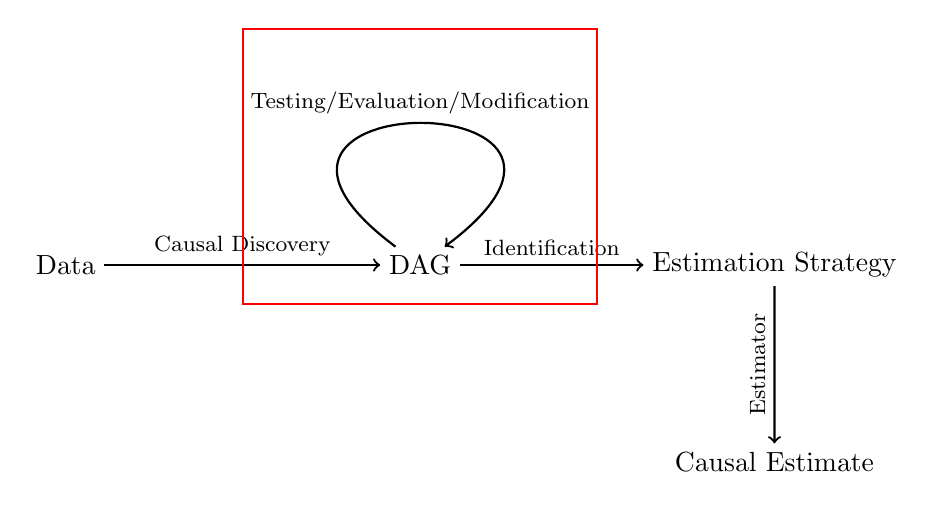
\begin{tikzpicture}[yscale=1, xscale=0.75, inner sep=3pt]
		\tikzstyle{every node}=[align=left]
			\node (data) at (0, 0) {Data};
			\node (dag) at (6, 0) {DAG};
			\node (estimand) at (12, 0) {Estimation Strategy};
			\node (estimation) at (12, -2.5) {Causal Estimate};
	
			\draw[thick, ->] (data) to node[midway, above]{\footnotesize Causal Discovery} (dag);
			\draw[thick, ->] (dag) to node[midway, above] {\footnotesize Identification} (estimand);
			\draw[thick, ->] (estimand) to node[midway, above, rotate=90] {\footnotesize Estimator} (estimation);
			\draw[thick, ->] (dag) [out=150, in=30, looseness=10] to node[midway, above] {\footnotesize Testing/Evaluation/Modification} (dag);

			\draw[draw=red, thick] (3, -0.5) rectangle (9, 3);
		\end{tikzpicture}
		\label{fig:workflow1}
	\end{figure}
\end{frame}

\begin{frame}{Model Evaluation}
	Even with integrating expert knowledge, how can we be sure? 
	As we have no ground truth information (think of unsupervised learning).
	
	\begin{itemize}
		\item Implied CIs: Benefits, local testing, gives a hint of where things are wrong.
		\item Fisher C: Similar to implied CIs but summerizes the whole model fit.
		\item Compare models using likelihood or a scoring metric to see which fits better.
	\end{itemize}
\end{frame}

\begin{frame}{Implied Conditional Independences (CIs)}

\end{frame}

\begin{frame}{Causal Discovery Algorithms learn a CPDAG}
	\begin{figure}
	\end{figure}
	
	\begin{itemize}
		\item Trying to learn a network structure which matches the covariance
			structure.
		\item Multiple networks can represent the same casual structure.
		\item Structure learning algorithms usually a DAG.
	\end{itemize}

	Pairwise edge orientation rules.
\end{frame}

\begin{frame}{Minimal Orientation}
\end{frame}

\begin{frame}{LLM Based Structure Learning}
	\begin{figure}
		\centering
		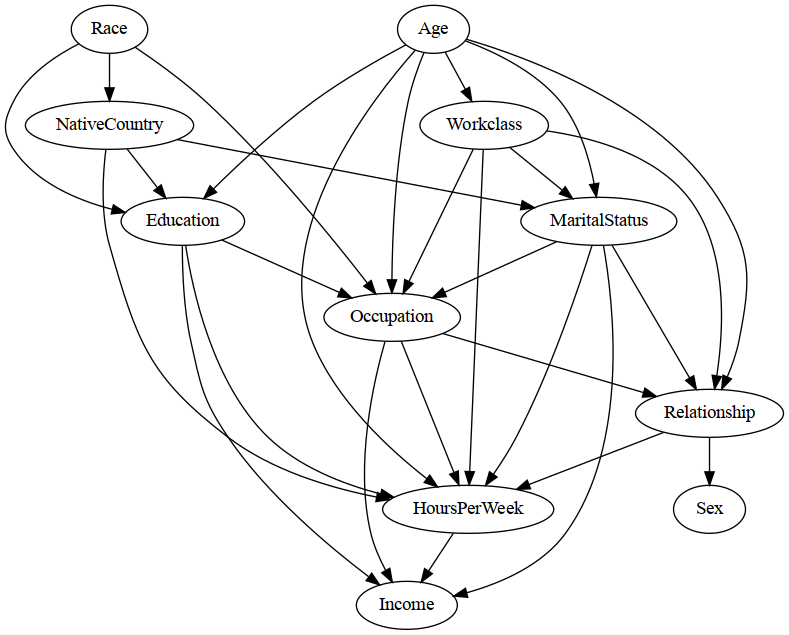
\includegraphics[scale=0.3]{imgs/adult_llm.png}
	\end{figure}
\end{frame}

\begin{frame}{Using DAG in the PO framework}
	As DAGs explicitly show all the information, it can be used to make
	decisions in the PO framework as well.

	The graph can be put into pywhy as well.
\end{frame}

\begin{frame}{Identification}
	\begin{itemize}
		\item Second step: Assuming that we have an oriented DAG.
		\item Everything is identified in the case of fully observed models.
		\item When latent variables are present, need to determine identfiablity.
	\end{itemize}
\end{frame}

\begin{frame}{do-calculus}
	\begin{itemize}
		\item Rules of do-calculus provide a full solution but no
			efficient algorithm.
		\item Other criterion with efficient algorithm but can only
			identify special cases.
		\item Back-door criterion
		\item Front-door criterion
		\item Instrumental variables.
	\end{itemize}
\end{frame}

\begin{frame}{Backdoor Criterion}
\end{frame}

\begin{frame}{Front-door Criterion}
\end{frame}

\begin{frame}{Instrumental Variables}
\end{frame}

\begin{frame}{pgmpy takes care of all this}
\end{frame}

\begin{frame}{Estimation}
	\begin{itemize}
		\item The identification method give the estimand.
		\item Use your favourite method for actual estimation.
	\end{itemize}
\end{frame}

\begin{frame}{Simulations}

\end{frame}

\begin{frame}{Extensible}
	\begin{itemize}
		\item Very active field of research, lots of new methods are getting developed.
		\item pgmpy offers easy ways to extend/modify algorithms where ever possible.
	\end{itemize}	
	$ random ci_test $
\end{frame}

\begin{frame}{Lot more functionality}
	\begin{itemize}
		\item Other models such as SEM, Dynamic Bayesian Networks, Cluster Graphs.
		\item Probabilistic Inference
		\item Approximate Inference using Sampling
		\item Reading writing to interface with other packages.
		\item Plotting functionality
		\item Parameter Estimation
	\end{itemize}
\end{frame}

\begin{frame}{Conclusion}
	\begin{itemize}
		\item Building causal models is an iterative process.
		\item Integrating expert knowledge can help a lot.
		\item Things are easy once we have the graph.
	\end{itemize}
\end{frame}

\begin{frame}{Future Plans}
	\begin{itemize}
		\item Focus on developing more practical methods.
		\item Wider support for mixed data.
	\end{itemize}
\end{frame}

\begin{frame}
	\center{\Huge {Thank you}}
	\vspace{5em}

	\github: pgmpy/pgmpy

	\email: ankurankan@gmail.com

	Consulting Company: Squanch Labs. Feel free to reach out to discuss use cases etc.
\end{frame}

\begin{frame}{Extra slide}
	When to use PO vs DAG framework?
\end{frame}

\begin{frame}
	How does it compare to Shapley values 
	\begin{itemize}
		\item Still prediction based. Does not matter if perturbing direct effect variable or undirect.
		\item Can show an example where Shapley values would still find an association, but causal inference would not. The standard confounding case.
	\end{itemize}
\end{frame}
\end{document}
